% STANDARD PACKAGES
\documentclass[a4paper, 11pt]{article}
\usepackage[utf8]{inputenc}
\usepackage[margin=2.5cm, bottom=3cm]{geometry}
% GRAPHEN
\usepackage{pgfplots}
\usepackage{graphicx}
\usepackage{pgfplotstable} 
\pgfplotsset{compat = 1.18, width=10cm}
% STYLING 
\usepackage{LocalDefs}
% FARBEN
\usepackage{xcolor,colortbl}
% MATHE
\usepackage{amsmath}
\usepackage{siunitx}   
% TABELLEN
\usepackage[thinlines]{easytable} % Zeilenhöhe
\usepackage{float} % Positionierung 
\usepackage{tabularx}
\usepackage{array}
\usepackage[table]{xcolor}
% FIGURES
\usepackage{subcaption}
\usepackage{tikz}
% CODE
\usepackage{listings}
% CITATIONS 
\usepackage{biblatex}
\addbibresource{Vortrag.bib}

\usepackage{fancyhdr}
\pagestyle{fancy}
\fancyhf{}
\renewcommand{\headrulewidth}{0pt}
\rfoot{\thepage}
\pagenumbering{arabic}


\usepackage{multicol}
% EXTRA COMMANDS
\newcommand{\todo}[1]{\textcolor{orange}{ToDo: #1}}
\newcommand{\evtl}[1]{\textcolor{blue}{Evtl.: #1}}
\newcommand{\gut}[1]{\textcolor{green}{Gut gemacht: #1}}
\newcommand{\com}[1]{\textcolor{gray}{Form und Layout: #1}}
\newcommand{\ant}[1]{\textcolor{gray}{Anmerkung: #1}}
\newcommand{\tcr}[1]{\textcolor{red}{#1}}
\newcommand{\tcw}[1]{\textcolor{white}{#1}}
\begin{document}

\Protokoll{zum Vortrag ''Minimizer-space de Bruijn-Graphen'' von Liliana Sanfilippo}{1}

\section{Einführung} 
Durch Technologien wie \textit{HiFi long read DNA sequencing} ist es möglich lange Reads mit niedrigen Fehlerraten herzustellen. Um aus derartigen Reads effizient Sequenzen oder ganze Genome assemblieren zu können, eignen sich klassische de Bruijn-Graphen nur bedingt, da der zeitliche Aufwand linear zu der Größe des Zielgenoms ist und sich bei Verzweigungen des Graphen durch Sequenzierfehler in den Reads sogar noch weiter erhöhen kann. Dies ist besonders bei fehleranfälligen Sequenziermethoden wie Nanopore ein Problem. 

De Bruijn-Graphen sind gewichtete, gerichtete Graphen, die zur Darstellung und Analyse von Sequenzen genutzt werden können. Dabei repräsentieren die Knoten $k$-mere und die Kanten Überlappungen der Länge $k-1$. 

Um das Problem langer Laufzeiten bei \textit{Whole Genome Assembly} zu adressieren, wurde von Baris Ekim, Bonnie Berger und Rayan Chikhi 2021 das Kommandozeilenprogramm \texttt{rust-mbdg} entwickelt. Als Basis dienen sogenannte \textit{Minimizer-Space-de-Bruijn-Graphen} (\textit{mdBG)}, die nur einen Teil der Basen einer Sequenz speichern, jedoch die Struktur der Sequenz erhalten. Dies ist durch sogenannte \textit{Minimizer} möglich, die 
%zu \textit{$k$-min-meren} zusammengesetzt 
$k$-mere komprimiert repräsentieren können. In diesem Format können die Sequenzen anschließend per de-Bruijn-Graphen assembliert werden. Durch 
%die Methode des \textit{partial order alignment} 
die implementierte Fehlerkorrektur können während der Assemblierung Sequenzierfehler teilweise korrigiert werden. 

Das Programm kann \texttt{FASTA}- und \texttt{FASTQ}-Dateien verarbeiten und produziert einen Sequenzgraphen im \texttt{GFA}-Format, sowie Sequenzdateien. 

\section{Methoden und Datenstrukturen}
\subsection{Minimizer und Minimizer-Raum}
Im Kontext von \textit{mdBG} bezeichnen \textit{Minimizer} nicht die klassischen lokalen Minimizer, die durch den lexikographisch kleinsten Teilstring einer bestimmten Länge eines $k$-mers bzw. eines Leserasters bestimmt sind. In diesem Fall handelt es sich um globale \textit{Minimizer}, die für alle betrachteten Reads festgelegt sind und sich je nach Wahl-Paramatern und Reads für jede Analyse unterscheiden können. 

Durch diese \textit{Minimizer} können Sequenzen über de-Bruijn-Graphen nicht nur als Abfolge von Basen (im Basen-Raum), sondern auch als Abfolge von \textit{Minimizern} (im \textit{Minimizer}-Raum) dargestellt werden. In den \textit{Minimizer}-Raum übersetzte $k$-mere werden als \textit{Minimizer}-$k$-mere bzw. \textit{$k$-min-mere} bezeichnet. Aus \textit{$k$-min-meren} bestehende de-Bruijn-Graphen werden als \textit{Minimizer-Space-de-Bruijn-Graphen} bezeichnet. 

Theoretisch ist es möglich Sequenzen ohne Informationsverlust vom Basen-Raum in den \textit{Minimizer}-Raum zu übersetzen und umgekehrt. Dafür müssen die \textit{Minimizer} jedoch passend gewählt werden. 

%Reprsäsentation durch ms

\subsubsection{Wählen der Minimizer}
\textit{Minimizer} sind Teilstrings einer Länge $l$ bestehend aus dem DNA-Alphabet. Dabei kommen nur Teilstrings in Frage, die in den Reads tatsächlich vorhanden sind. Weiterhin darf es nur eine Begrenzte Anzahl an \textit{Minimizern} geben und jene dürfen durchschnittlich weder zu häufig, noch zu selten in den Reads vorkommen. 

Die Anzahl wird durch einen als Dichte $\delta$ bezeichneten Koeffizienten begrenzt. Je nach Zielgenom können sich die Parameter für $l$ und $\delta$, sowie die obere und untere Grenze der Häufigkeit, unterscheiden und sie können nicht pauschal festgelegt werden, sondern müssen experimentell ermittelt und verifiziert werden. 

Um die aus \textit{$k$-min-meren} bestehende Sequenz nach Abschluss der Assemblierung im \textit{Minimizer}-Raum zurück in den Basen-Raum übersetzen zu können, wird für jedes \textit{$k$-min-mer} das entsprechende $k$-mer gespeichert. 
%Wichtig: Zuordnung der k-mere zu  den k-min meren wird gespeichert
%Universe-Minimizer werden hier verwendet (Menge von l-meren mit bestimmten Bedingungen und niedrigen Hash-Werten)
%Es gibt auch Window-Minimizer, das ist eher die klassische Definition (kleinstes l-mer in einem Fenster, das weiter geschoben wird) 
%außerdem speichern wir die Reihenfolge der Minimizer pro Read, also ordnen Reads und minimizer zu
\paragraph{1. Wählen der Parameter} Trivialerweise muss $l$ kleiner sein als die kürzeste Read-Länge. Für die von den Autoren durchgeführten Experimente wurden Werte von 10 bis 14 gewählt.

Wird die Dichte zu niedrig gewählt, gibt es möglicherweise nicht genug Minimizer, um alle $k$-mere eindeutig aus dem \textit{Minimizer}-Raum zurück in den Basen-Raum übersetzen zu können. Eine zu hohe Dichte kann zur Folge haben, dass Effizienz eingebüßt wird, da die $k$-mere ebenso durch weniger \textit{Minimizer} eindeutig hätten übersetzt werden können.  

\paragraph{2. K-mere identifizieren und zählen} Im ersten Schritt der \textit{Minimizer}-Wahl werden alle kanonischen $l$-mere der Reads identifiziert und ihre Vorkommen werden gezählt. 

\paragraph{3. Obere und untere Grenze} Es werden ausschließlich $l$-mere in Betracht gezogen, die innerhalb der festgelegten oberen und unteren Grenze der akzeptierten Häufigkeit liegen. 

\paragraph{4. K-mere hashen und normalisieren} Es werde alle $l$-mere in Zahlenwerte gehasht und diese Werte auf ein Intervall $[0,1]$ normalisiert. 

\paragraph{5. Begrenzung der Anzahl durch die Dichte}
Alle $l$-mere, deren normalisierte Hashwerte kleiner sind als die festgelegte Dichte $\delta$, werden als \textit{Minimizer} akzeptiert. 


\subsection{Fehlerkorrektur}
Sequenzierfehler wie Insertionen, Deletionen oder Substitutionen können verschieden schwere Auswirkungen auf die Übersetzung von $k$-meren in \textit{$k$-min-mere} haben. Es können \textit{Minimizer} in der \textit{$k$-min-meren} hinzukommen, ausgetauscht werden oder wegfallen. Bei vielen Fehlern ist es theoretisch möglich, dass ein fehlerhaftes $k$-mer in ein \textit{$k$-min-mer} übersetzt würde, das keinen \textit{Minimizer} mit dem \textit{$k$-min-mer} des tatsächlichen $k$-mers gemeinsam hat (siehe Beispiel in Tab. \ref{tab:reads}). 

Um mit Sequenzierdaten von fehleranfälligen Technologien ($> 1\%$ Fehlerrate) arbeiten zu können, muss daher eine Fehlerkorrektur vorgenommen werden. Dies geschieht durch Filterung und \textit{partial order alignment} von Reads. Bei wird ein Read als \textit{Query-Read} verwendet, um zusammen mit weiteren Reads die unbekannte tatsächliche Sequenz zu ermitteln. 

\begin{table}[H]
    \centering
    \small
\(
  \begin{array}{|l | ccccccccccccccc | l | } \hline
       \text{Tatsächliche} &  \textbf{A} &  \textbf{C} & \text{G} & \text{G}  & \textbf{A} & \textbf{T} & \text{T} & \text{C} & & \text{C} & \text{G}  & \text{G}  & \textbf{A} & \textbf{A} & &    \\ 
       \text{Sequenz}&  \multicolumn{2}{c}{m1} & & & \multicolumn{2}{c}{m2}  & & &  & & &  & \multicolumn{2}{c}{m3} & & \\ \hline \hline
     \text{Query-Read} &  \textbf{A} &  \textbf{C} & \text{G} & \text{G}  & \textbf{A} & \textbf{T} & \text{T} & \text{C} & \textbf{\tcr{A}} & \textbf{C} & \text{G}  & \text{G}  & \textbf{A} & \textbf{A} & &
     \\ 
      &  \multicolumn{2}{c}{m1} & & & \multicolumn{2}{c}{m2}  & & & \multicolumn{2}{c}{\tcr{m1}}  &  & \multicolumn{2}{c}{m3} & &  & 
      \ \  m1 \ \tcw{m4} \ \tcw{m4} \ m2       \ \tcr{m1} \ m3 \ \tcw{m4} 
      \\ \hline \hline
      \text{Read 1} &  \textbf{A} &  \textbf{C} & \text{G} & \text{G}  & \textbf{A} & \textbf{T} & \text{T} & \text{C} & & \text{C} & \text{G}  & \text{G}  & \textbf{A} & \textbf{A} & \textbf{\tcr{T}} & \\
       &  \multicolumn{2}{c}{m1} & & & \multicolumn{2}{c}{m2}  & & &  & & &  & \multicolumn{3}{c|}{m3 $\ \ \ $ \tcr{m2}} 
       &  \   \  m1 \ \tcw{m4} \ \tcw{m4} \ m2       \ \tcw{m1} \ m3 \ \tcr{m2}  \\
       \hline \hline
\text{Read 2} &  \textbf{A} &  \textbf{C} & \textbf{\tcr{A}} & \textbf{G}  & \textbf{A} & \textbf{T} & \text{T} & \text{C} & & \text{C} & \text{G}  & \text{G}  & \textbf{A} & \textbf{A} && \\
&  \multicolumn{2}{c}{m1} &  \multicolumn{2}{c}{\tcr{m4}} & \multicolumn{2}{c}{m2}  & & &  & & &  & \multicolumn{2}{c}{m3} & & 
\      \ m1 \ \tcw{m4} \ \tcr{m4} \ m2       \ \tcw{m1} \ m3 \ \tcw{m4}
\\ \hline \hline
\text{Read 3} &  \textbf{A} &  \textbf{\tcr{A}} & \textbf{G} & \text{G}  & \tcr{\_} & \text{T} & \text{T} & \text{C} & & \text{C} & \text{G}  & \text{G}  & \textbf{A} & \textbf{A} && \\
 &  \multicolumn{3}{c}{\tcr{m3} $\ \ \ $ \tcr{m4}}  & &\multicolumn{2}{c}{\tcr{-}}  & & &  & & &  & \multicolumn{2}{c}{m3} & &
 \ \ \tcr{m3}  \ \tcr{m4} \ \tcw{m4} \  \ \tcr{-} \ \ \tcw{m1} \ m3 \ \tcw{m4} 
 \\ \hline \hline
\text{Read 4} &  \textbf{A} &  \tcr{\_}  & \textbf{G} & \text{G}  & \tcr{\_}  & \text{T} & \text{T} & \text{C} & & \text{C} & \text{G}  & \text{G}  & \textbf{A} & \textbf{\tcr{G}} &&\\
 &  \multicolumn{3}{c}{\tcr{m4}}  & & \multicolumn{2}{c}{\tcr{-}} & & &  & & &  & \multicolumn{2}{c}{\tcr{m4}}  & &
 \  \ \  \ \ \tcr{m4} \ \ \ \tcw{m4}  \ \ \tcr{-} \ \ \tcw{m1} \ \tcr{m4} \ \tcw{m4}
 \\ \hline
    \end{array}
\)
    \caption{Caption}
    \label{tab:reads}
\end{table}

Dafür werden zuerst Reads herausgefiltert, die keine Ähnlichkeit zu dem \textit{Query-Read} haben. Beim \textit{Minimizer Bucketing} werden die weiteren Reads bezüglich der einzelnen im \textit{Query-Read} enthaltenen \textit{Minimizer} gruppiert (Siehe Beispiel Tab. \ref{tab:buckets}). Reads, die keinen \textit{Minimizer} mit der \textit{Query-Sequenz} gemeinsam haben, werden nicht gruppiert und in weiteren Schritten nicht einbezogen. 

\begin{table}[H]
    \centering
    \footnotesize
\(
\begin{array}{|l | cccccc | cccccc | ccccccc|} \hline
 & \multicolumn{6}{c|}{\mathbf{m1}\textbf{-Bucket}} &  \multicolumn{6}{c|}{\mathbf{m2}\textbf{-Bucket}} &  \multicolumn{7}{c|}{\mathbf{m3}\textbf{-Bucket}}\\ \hline
 \text{QR}:& m1 & & m2 & \tcr{m1} & m3 & & m1 & & m2 & \tcr{m1} & m3 & & m1 & && m2 & \tcr{m1} & m3 & \\ 
  \text{R1}:& m1 & & m2 & & m3  & \tcr{m4} & m1 & & m2 & & m3  & \tcr{m4}  & m1 & & &m2 & & m3  & \tcr{m4}  \\
  \text{R2}:&   m1& \tcr{m4} & m2 & & m3 & &   m1 & \tcr{m4} & m2 & & m3 &  &   m1 && \tcr{m4} & m2 & & m3 &   \\
   \text{R3}: &&&&&&&&&&&& &   \tcr{m3} & \tcr{m4} & &  \tcr{-} & & m3 &  \\ \hline
\end{array}
\)
    \caption{Caption}
    \label{tab:buckets}
\end{table}
\normalsize

Im nächsten Schritt werden Reads herausgefiltert, die keine ausreichende Ähnlichkeit zu dem \textit{Query-Read} haben. 

\begin{figure}[H]
    \centering
    \begin{subfigure}[t]{0.3\linewidth}
    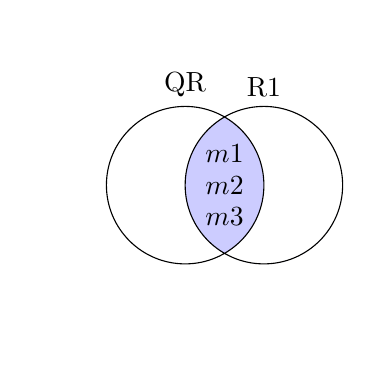
\begin{tikzpicture}[fill=white]
% left hand
\scope
\clip (-2,-2) rectangle (2,2);
\fill[blue!20] (1,0) circle (1);
 (0,0) circle (1);
\endscope
% right hand
\scope
\clip (-2,-2) rectangle (2,2)
   (0,0) circle (1);
 \fill (1,0) circle (1);
\endscope
% outline
\draw (0,0) circle (1) (0,1)  node [text=black,above] {QR}
      (1,0) circle (1) (1,1)  node [text=black,above] {R1};
\node at (0.5,0.4) {$m1$};
\node at (0.5,0) {$m2$};
\node at (0.5,-0.4) {$m3$};
\end{tikzpicture}
     \caption{Caption}
    \label{fig:my_label}
    \end{subfigure}
    \hfill
     \begin{subfigure}[t]{0.3\linewidth}
     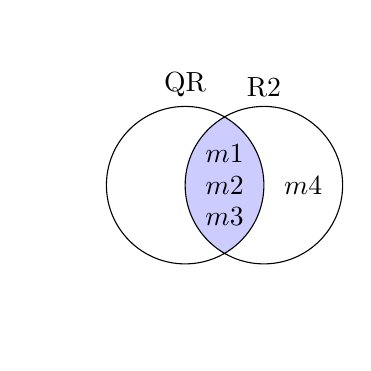
\begin{tikzpicture}[fill=white]
% left hand
\scope
\clip (-2,-2) rectangle (2,2) ;
\fill[blue!20] (1,0) circle (1);
 (0,0) circle (1);
\endscope
% right hand
\scope
\clip (-2,-2) rectangle (2,2)
   (0,0) circle (1);
 \fill (1,0) circle (1);
\endscope
% outline
\draw (0,0) circle (1) (0,1)  node [text=black,above] {QR}
      (1,0) circle (1) (1,1)  node [text=black,above] {R2};
\node at (0.5,0.4) {$m1$};
\node at (0.5,0) {$m2$};
\node at (0.5,-0.4) {$m3$};
\node at (1.5,0) {$m4$};
\end{tikzpicture}
 \caption{Caption}  
    \label{fig:my_label}
    \end{subfigure}
    \hfill
    \begin{subfigure}[t]{0.3\linewidth}
    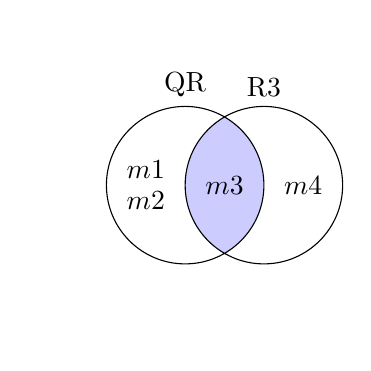
\begin{tikzpicture}[fill=white]
% left hand
\scope
\clip (-2,-2) rectangle (2,2) ;
\fill[blue!20] (1,0) circle (1);
 (0,0) circle (1);
\endscope
% right hand
\scope
\clip (-2,-2) rectangle (2,2)
   (0,0) circle (1);
 \fill (1,0) circle (1);
\endscope
% outline
\draw (0,0) circle (1) (0,1)  node [text=black,above] {QR}
      (1,0) circle (1) (1,1)  node [text=black,above] {R3};
\node at (-0.5,0.2) {$m1$};
\node at (0.5,0) {$m3$};
\node at (-0.5,-0.2) {$m2$};
\node at (1.5,0) {$m4$};
\end{tikzpicture}
     \caption{Caption}
    \label{fig:my_label}
    \end{subfigure}
    \caption{Caption}
    \label{fig:my_label}
\end{figure}


\begin{figure}[H]
    \centering
   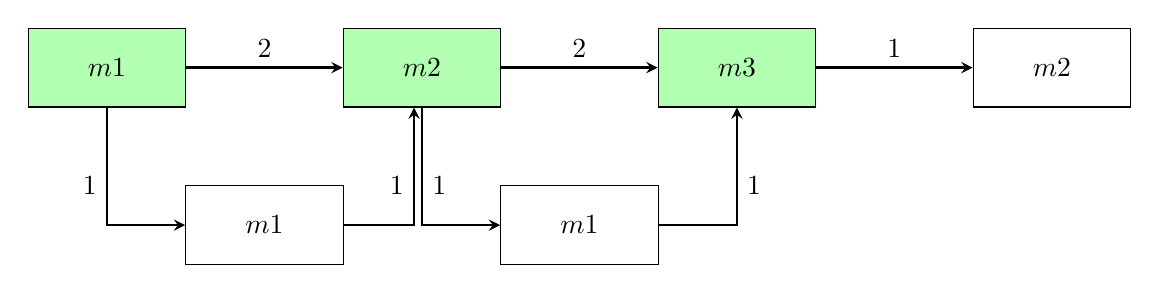
\begin{tikzpicture}[node distance=2cm]
   \tikzstyle{consensus} = [rectangle, minimum width=2cm, minimum height=1cm, text centered, draw=black, fill=green!30]
\tikzstyle{normalnode} = [rectangle, minimum width=2cm, minimum height=1cm, text centered, draw=black, fill=white]
\tikzstyle{filler} = [rectangle, minimum width=2cm, minimum height=1cm, text centered, draw=white, fill=white]

\tikzstyle{arrow} = [thick,->,>=stealth]

\node (m1) [consensus] {$m1$};
\node (lam2) [filler, right of=m1, xshift=1.9cm] {};
\node (m2) [consensus, right of=m1, xshift=2cm] {$m2$};
\node (m3) [consensus, right of=m2, xshift=2cm] {$m3$};
\node (fm2) [normalnode, right of=m3, xshift=2cm] {$m2$};

\node (fm1) [normalnode, below of=m1, xshift=2cm] {$m1$};
\node (ffm1) [normalnode, below of=m2, xshift=2cm] {$m1$};

\draw [arrow] (m1) -- node[anchor=south] {2} (m2);
\draw [arrow] (m2) -- node[anchor=south] {2} (m3);
\draw [arrow] (m3) -- node[anchor=south] {1} (fm2);

\draw [arrow] (m1) |-  node[anchor=east, yshift=0.5cm] {1} (fm1);
\draw [arrow] (fm1) -|  node[anchor=east, yshift=0.5cm] {1} (lam2);

\draw [arrow] (m2) |-  node[anchor=west, yshift=0.5cm] {1} (ffm1);
\draw [arrow] (ffm1) -|  node[anchor=west, yshift=0.5cm] {1} (m3);
   \end{tikzpicture}
    \caption{Caption}
    \label{fig:my_label}
\end{figure}




\subsection{Assembly}

\subsection{Rekonstruktion}

\section{Effizienz und Qualität}
\subsection{Laufzeit und Speicherkomplexität}
D. Melanogaster

PacBio HiFi reads (highly accurate long reads) 

Simulated perfect reads (künstlich erstellte, korrekte reads), generell zum Testen von Bioinformatik Tools
Minimizer machen es skalierbar 

\begin{figure}[H]
    \centering
  \begin{subfigure}[t]{0.49\linewidth} 
  \centering
    \pgfplotstableread[row sep=\\,col sep=&]{
    interval & 100Hifi & 50sim \\
    Rust-mdbg & 1.5  & 1    \\
    Hifiasm   & 21 & 51 \\
    HiCanu    &12 & 18  \\
    Peregrine  & 12 &16 \\
    }\mydata
   \begin{tikzpicture}
   \begin{axis}[
    ybar,
    bar width=0.5cm,
    width=\textwidth,
    height=8cm,
    enlarge x limits=0.2,
    ylabel={Speicher (GB)},
    symbolic x coords={Rust-mdbg,Hifiasm,HiCanu,Peregrine},
    xtick=data,
    bar shift auto,
    legend style={at={(0.5,-0.15)}, anchor=north, legend columns=-1},
    nodes near coords,
]
   symbolic x coords={Rust-mdbg,Hifiasm,HiCanu,Peregrine},]
\addplot table[x=interval,y=100Hifi]{\mydata};
\addplot table[x=interval,y=50sim]{\mydata};
\end{axis}
   \end{tikzpicture}
    \caption{Caption}
    \label{fig:my_label}
  \end{subfigure}
  \hfill
  \begin{subfigure}[t]{0.49\linewidth}
  \centering
    \pgfplotstableread[row sep=\\,col sep=&]{
    interval & 100Hifi & 50sim \\
    Rust-mdbg & 1  & 0.2    \\
    Hifiasm   & 317 & 1178 \\
    HiCanu    &462 & 492  \\
    Peregrine  & 40 & 23 \\
    }\mydata
   \begin{tikzpicture}
   \begin{axis}[
    ybar,
    bar width=0.5cm,
    width=\textwidth,
    height=8cm,
    enlarge x limits=0.2,
    ylabel={Zeit (Min)},
    symbolic x coords={Rust-mdbg,Hifiasm,HiCanu,Peregrine},
    xtick=data,
    bar shift auto,
    legend style={at={(0.5,-0.15)}, anchor=north, legend columns=-1},
    nodes near coords,
]
   symbolic x coords={Rust-mdbg,Hifiasm,HiCanu,Peregrine},]
\addplot table[x=interval,y=100Hifi]{\mydata};
\addplot table[x=interval,y=50sim]{\mydata};
\end{axis}
   \end{tikzpicture}
    \caption{Caption}
    \label{fig:my_label}
  \end{subfigure}
   \caption{Caption}
    \label{fig:my_label}
\end{figure}
\subsection{Qualität}
1: D. melanogaster chromosome 4  wurden mit versch. Error-Raten simuliert (Read error rate)

Unter 5\% Error Rate ist gut  (ist 1.2 Mb lang)

2: Read identity to the reference – wie ähnlich der rekonstruierte Read zu der tatsächlichen Sequenz (Referenzsequenz) ist  


\section{Limitationen}
Abhängigkeit von den Minimizer-Paramatern
• Keine Vorkorrektur (Polishing)
• Unterscheidung zwischen Haplotypen nicht möglich
• Potentiell Probleme mit Nanopore-Daten

\section{Ausblick}
Metagenome Assembly (metaMDBG)
oMetagenome assembly from nanopore reads (nanoMDBG)
• Mapping of accurate long reads (mapquik)
• Pangenome Graphen (MDBG allg.) \cite{meta} \cite{nano} \cite{mainpaper} \cite{github}


\printbibliography
\end{document}